\documentclass[UTF8]{ctexart}
\usepackage{xcolor}
\usepackage{enumerate}
\usepackage{graphicx}
\usepackage{geometry}
\usepackage{graphicx} %插入图片的宏包
\usepackage{float} %设置图片浮动位置的宏包
\usepackage{subfigure} %插入多图时用子图显示的宏包
\geometry{left = 2.5cm,right= 2cm}
\title{Sketch of Chapter 1}
\author{DuLi}
\date{\today}
\begin{document}
\maketitle
\newpage
\tableofcontents
\newpage
\section{Definition of Machine Learning}
\subsection{Arthur Samuel's Definition}
\setlength{\parskip}{0.5em} 

\large \textbf{\emph{Machine Learning is a field of study that gives computers the ability to learn without being explicitly programmed.}}

这个定义看来是非常general了,基本上是从字面上解释了这个词组。稍微提一下Arthur Samuel这个人,直接把Wikipedia的简介搬过来。大体就是上古大神的意思了。

\begin{figure}[H]
\centering
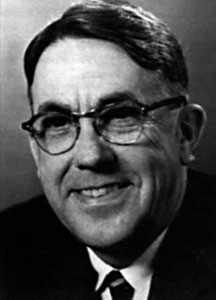
\includegraphics[width = 1.3in]{This_is_the_photo_of_Arthur_Samuel.jpg}
\caption{Arthur Samuel}
\end{figure}

Arthur Lee Samuel (December 5, 1901 – July 29, 1990)was an American pioneer in the field of computer gaming and artificial intelligence.He coined the term "machine learning" in 1959.The Samuel Checkers-playing Program was among the world's first successful self-learning programs, and as such a very early demonstration of the fundamental concept of artificial intelligence (AI).He was also a senior member in the TeX community who devoted much time giving personal attention to the needs of users and wrote an early TeX manual in 1983.

\subsection{Tom Michell's definition}
\large \textbf{A computer program is said to learn from experience E with respect to some task T and some performance measure P,if its performance on T,as measured by P,improves with experience E.}

乍一看这个写的比较拗口,但实际上也就是说通过对experience E的学习,使原有task T的performance P有了提高。对于Tom Michell的了解大概是因为那本机器学习的教材,薄薄一本,当时应该是看过同学的,没有看太多,也不好评价。这个定义就显得更像在描述一个事情而非定义。本书接下来用一个简单的例子来说明了一下,那就是spam filter,并将Tom Michell的定义套用做了讲解。
\begin{figure}[H]
\centering
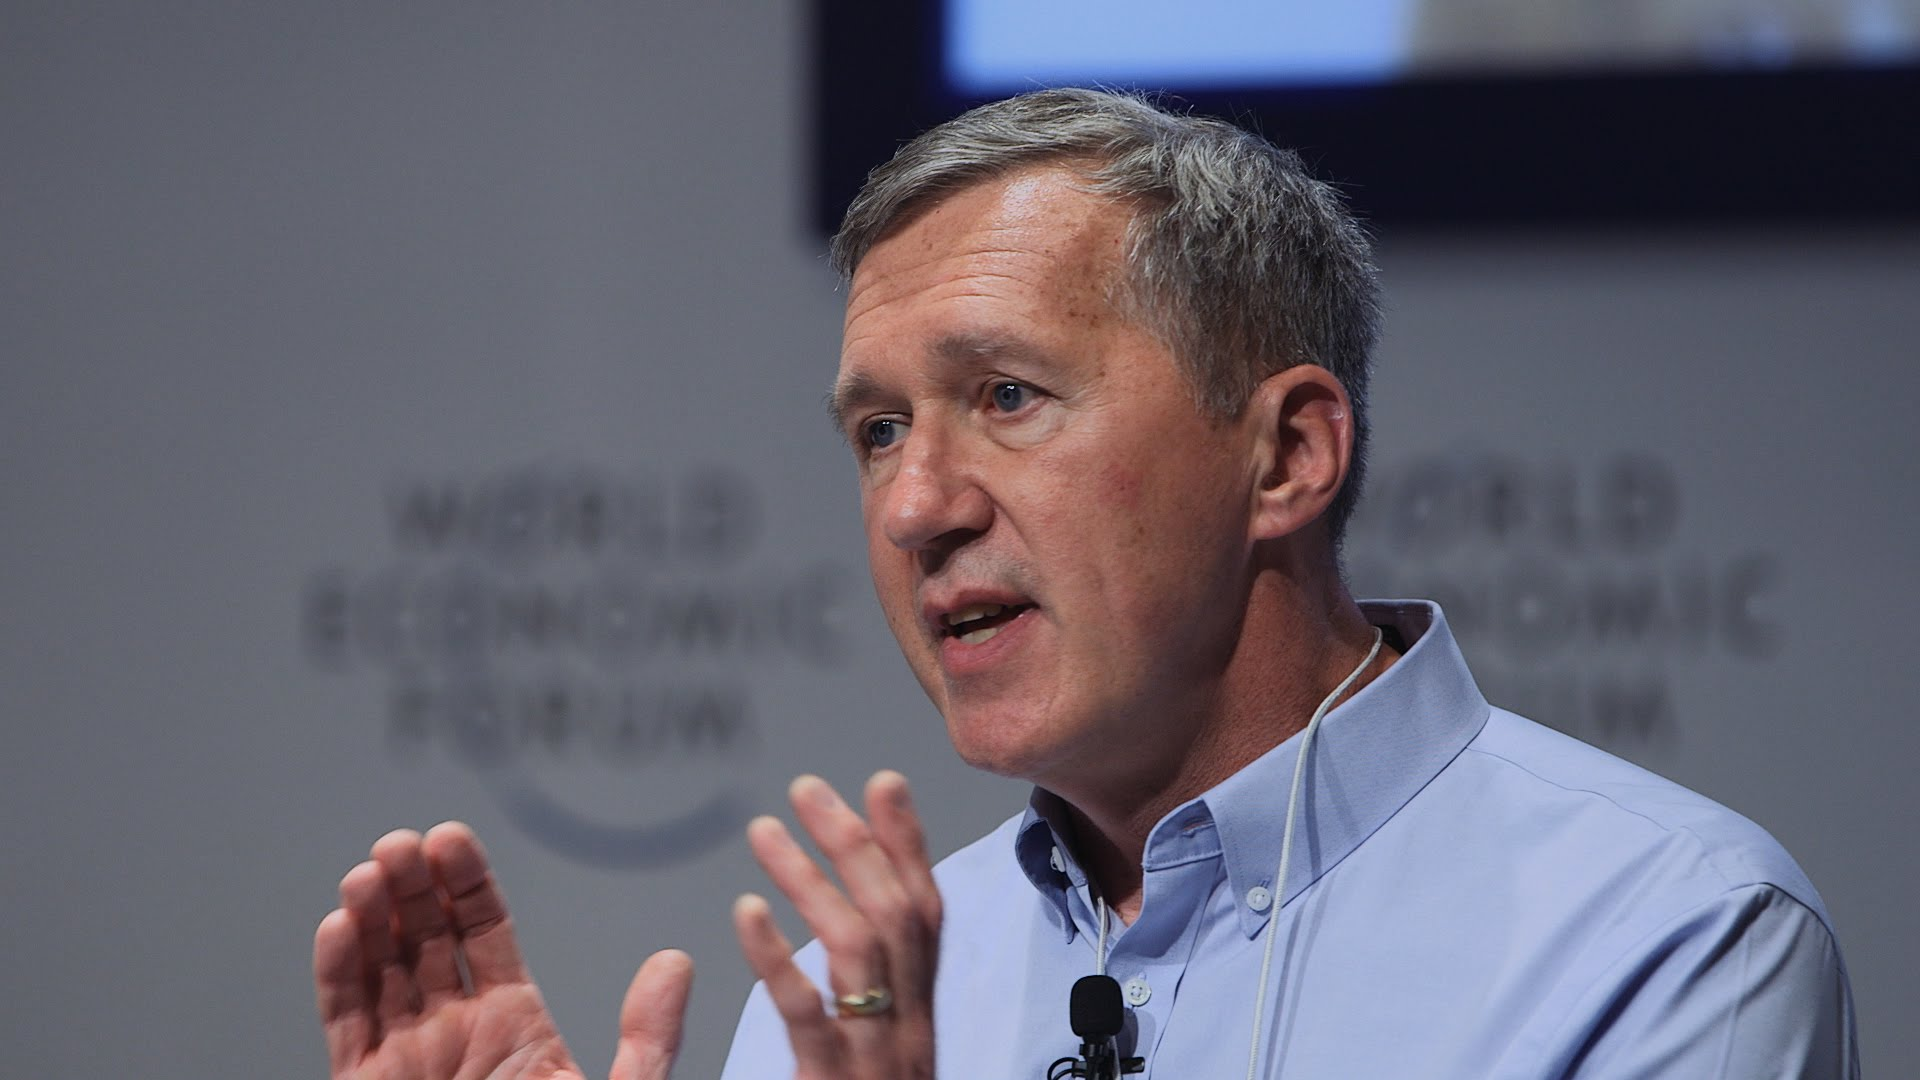
\includegraphics[width = 2in]{TomWEF2017.jpg}
\caption{Tom Michell}
\end{figure}

\section{Why use Machine Learning}
依旧以写一个spam filter为例,当使用传统的编程技术时,需要一个长长的规则清单,并且这个规则是难以把握且复杂的。相反,当使用Machine Learning Techniques时,可以让机器自主的学习知识,学习垃圾邮件中的词频,这显然更加简洁高效。To summarize,Machine Learning is great for:
\begin{enumerate}

\item Problems require a lot of hand-tuning or long list of rules.

\item Complex problems is no good solution using traditional approach.

\item Fluctuating enviornment

\item Getting insights about complex problems and large amount of data
\end{enumerate}

\subsection{Types of Machine Learning Systems}
\begin{itemize}
	\item[-] Whether or not they are trained with human supervision(Supervised Unsupervised Semisupervised Reinforcement Learning 监督 非监督 半监督 强化学习)

	\item[-] Whether or not they can learn incrementally(Online versus Batch learning 在线学习 VS 批量学习)

	\item[-] Whether work by comparing new data to  known data or instead detect patterns in the training data and build a predictive model(instance-based versus model-based learning 基于模型 vs 基于实例)

\end{itemize}

\section{Supervised/Unsupervised Learning}
\subsection{Supervised Learning}

The training data you feed to the algorithm includes the desire solutions,called \emph{labels}.Here are some most important supervised learning algorithms(在后文中都有体现):

\begin{itemize}
	\item[-] k-Nearest Neighbors
	\item[-] Linear Regression
	\item[-] Logistic Regression
	\item[-] Support Vector Machines
	\item[-] Decision Trees and Random Forests
	\item[-] Neural networks
\end{itemize}

\subsection{Unsupervised Learning}

The training data is unlabeled.Some important unsupervised learning algorithms:
\begin{itemize}
	\item Clustering
	\item[-] k-Means
	\item[-] Hierarchical Cluster Analysis(HCA)
	\item[-] Expection Maximization
	\item Visualization and dimensionality reduction
	\item[-] Principle Component Analysis(PCA)
	\item[-] Kernel PCA
	\item[-] Locally-Linear Embedding(LLE)
	\item[-] t-distributed Stochastic Neighbor Embedding(t-SNE)
	\item Associaton rule learning
	\item[-] Apriori
	\item[-] Eclat
\end{itemize}

\subsection{Reinforcement Learning}





\end{document}